\documentclass[letterpaper,11pt]{article}

\usepackage{latexsym}
\usepackage[empty]{fullpage}
\usepackage{titlesec}
\usepackage{marvosym}
\usepackage[usenames,dvipsnames]{color}
\usepackage{verbatim}
\usepackage{enumitem}
\usepackage[hidelinks]{hyperref}
\usepackage{fancyhdr}
\usepackage[english]{babel}
\usepackage{tabularx}
\usepackage{fontawesome5}
\usepackage{multicol}
\setlength{\multicolsep}{-3.0pt}
\setlength{\columnsep}{-1pt}
\input{glyphtounicode}

%new packages

\usepackage{fontenc}
\usepackage{amsmath}
\usepackage{amssymb}
\usepackage{graphicx}



%----------FONT OPTIONS----------

\pagestyle{fancy}
\fancyhf{} % clear all header and footer fields
\fancyfoot{}
\renewcommand{\headrulewidth}{0pt}
\renewcommand{\footrulewidth}{0pt}

% Adjust margins
\addtolength{\oddsidemargin}{-0.6in}
\addtolength{\evensidemargin}{-0.5in}
\addtolength{\textwidth}{1.19in}
\addtolength{\topmargin}{-.7in}
\addtolength{\textheight}{1.4in}

\urlstyle{same}

\raggedbottom
\raggedright
\setlength{\tabcolsep}{0in}

% Sections formatting
\titleformat{\section}{
  \vspace{-4pt}\scshape\raggedright\large\bfseries
}{}{0em}{}[\color{black}\titlerule \vspace{-5pt}]



% Ensure that generate pdf is machine readable/ATS parsable
\pdfgentounicode=1

%-------------------------
% Custom commands
\newcommand{\resumeItem}[1]{
  \item\small{
    {#1 \vspace{-2pt}}
  }
}

\newcommand{\classesList}[4]{
    \item\small{
        {#1 #2 #3 #4 \vspace{-2pt}}
  }
}

\newcommand{\resumeSubheading}[4]{
  \vspace{-2pt}\item
    \begin{tabular*}{1.0\textwidth}[t]{l@{\extracolsep{\fill}}r}
      \textbf{#1} & \textbf{\small #2} \\
      \textit{\small#3} & \textit{\small #4} \\
    \end{tabular*}\vspace{-7pt}
}

\newcommand{\resumeSubSubheading}[2]{
    \item
    \begin{tabular*}{0.97\textwidth}{l@{\extracolsep{\fill}}r}
      \textit{\small#1} & \textit{\small #2} \\
    \end{tabular*}\vspace{-7pt}
}

\newcommand{\resumeProjectHeading}[2]{
    \item
    \begin{tabular*}{1.001\textwidth}{l@{\extracolsep{\fill}}r}
      \small#1 & \textbf{\small #2}\\
    \end{tabular*}\vspace{-7pt}
}


\newcommand{\resumeSubItem}[1]{\resumeItem{#1}\vspace{-4pt}}

\renewcommand\labelitemi{$\vcenter{\hbox{\tiny$\bullet$}}$}
\renewcommand\labelitemii{$\vcenter{\hbox{\tiny$\bullet$}}$}

\newcommand{\resumeSubHeadingListStart}{\begin{itemize}[leftmargin=0.0in, label={}]}
\newcommand{\resumeSubHeadingListEnd}{\end{itemize}}
\newcommand{\resumeItemListStart}{\begin{itemize}}
\newcommand{\resumeItemListEnd}{\end{itemize}\vspace{-5pt}}

\begin{document}
\fontfamily{cmr}\selectfont
\begin{center}
\parbox{3.0cm}{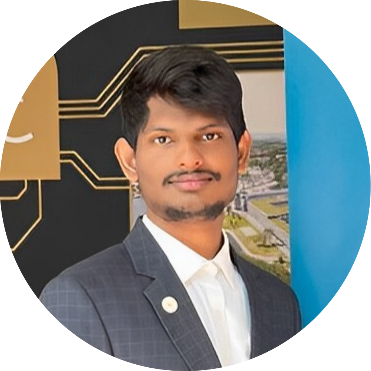
\includegraphics[width=2.7cm,clip]{images/resume_pic_m.png}}
\parbox{\dimexpr\linewidth-3.8cm\relax}{
\vspace{-20pt}
\begin{tabularx}{\linewidth}{L r} \\
    {\Huge \scshape  Venkata Sai Yakkshit Reddy Asodi}~\\
      Berlin, Germany. \\ \vspace{1pt}
     \small \raisebox{-0.1\height}\faPhone\ +91 8179936156 ~ \href{mailto:saiyakkshit2001@gmail.com}{\raisebox{-0.2\height}\faEnvelope\  {saiyakkshit2001@gmail.com}} ~ 
    \href{https://linkedin.com/in/yakkshit/}{\raisebox{-0.2\height}\faLinkedin\ {yakkshit}}  ~
    \href{https://yakkshit.com/}{\raisebox{-0.2\height}\faGlobe\ {yakkshit.com}}  ~
    \href{https://github.com/yakkshit}{\raisebox{-0.2\height}\faGithub{ yakkshit}}
    \vspace{-8pt}
\end{tabularx}
}
\end{center}

\vspace{-23pt}
%-----------EDUCATION-----------
\section{Summary}
Dynamic Full Stack Developer with extensive experience building AI-driven web applications. Proven track record in integrating APIs, optimizing performance, and delivering high-quality, maintainable code. Passionate about personal growth, scalability, and AI technologies in property management solutions.

%-----------PROGRAMMING SKILLS-----------
\section{Technical Skills}
\begin{itemize}[leftmargin=0.15in, label={}]
\small{\item{
\textbf{Frameworks - }{React, Next.js, Node.js, Django, Express.js, TailwindCSS, Figma.} \\
\textbf{Languages - }{JavaScript, TypeScript, Python, SQL.} \\
\textbf{Tools - }{Git, Docker, Postman, Swagger, RESTful APIs.} \\
\textbf{Cloud - }{AWS, Azure, Firebase, Google Cloud.}\\
}}
\end{itemize}
\vspace{-10pt}

%-----------EXPERIENCE-----------
\section{Experience}
\resumeSubHeadingListStart

\resumeSubheading
{Circleup AG}{Jan 2024 -- Present}
{Lead Full Stack Engineer}{Zurich, Switzerland}\\
\vspace{10pt}
\textbf{Responsibilities:}
\resumeItemListStart
\vspace{-10pt}
\resumeItem{Developing AI-driven features for property management software with seamless API integrations.}
\resumeItem{Ensured high-quality, scalable code by conducting thorough code reviews and performance testing.}
\resumeItem{Led the design and implementation of reusable front-end components, improving development speed and quality.}
\resumeItemListEnd
\vspace{-3pt}
\textbf{Environment:} \emph{React, TypeScript, Django, PostgreSQL, AWS, Docker, LLMs, OpenAI API.}

\resumeSubheading
{Cedzlabs}{Aug 2022 -- Dec 2023}
{Full Stack Developer}{India}\\
\vspace{10pt}
\textbf{Responsibilities:}
\vspace{-10pt}
\resumeItemListStart
\resumeItem{Developed full-stack applications using React, Node.js, and Firebase, ensuring cross-platform compatibility.}
\resumeItem{Led migration of legacy systems to modern, scalable web services using cloud-based solutions.}
\resumeItemListEnd
\vspace{-3pt}
\textbf{Environment:} \emph{React, Node.js, Firebase, Docker, Git, JavaScript.}

%-----------PROJECTS-----------
\section{Projects}
\resumeSubHeadingListStart
\resumeProjectHeading
{\textbf{AI Property Manager} $|$ \emph{Next.js, Node.js, OpenAI API, Firebase}}{Mar 2024 -- Present}\\
\vspace{6pt}
\textbf{Description:}
\vspace{-5pt}
\resumeItemListStart
\resumeItem{Developed an AI-powered property management platform to automate tenant communication, using OpenAI's GPT APIs for generating personalized responses and integrating Firebase for real-time updates.}
\resumeItemListEnd
\vspace{4pt}
\textbf{Tools:} \emph{Next.js, Firebase, OpenAI API, Node.js.}

\resumeProjectHeading
{\textbf{AI Resume Tuner} $|$ \emph{Azure Cloud, Next.js, RAG, LLMs}}{Aug 2023}\\
\vspace{6pt}
\textbf{Description:}
\vspace{-5pt}
\resumeItemListStart
\resumeItem{Developed an AI-powered resume tuning tool that generates tailored resumes based on job descriptions and user input, leveraging LLMs and deployed on Azure.}
\resumeItemListEnd
\vspace{4pt}
\textbf{Tools:} \emph{Next.js, Azure, LLMs, RAG.}

%-----------ACHIEVEMENTS-----------
\section{Achievements}
\begin{itemize}
\item Successfully optimized tenant communication by integrating AI-powered systems, reducing response times by 30\%.
\item Led the development of scalable full-stack applications for over 400+ tenants using React and Firebase.
\item Contributed to open-source projects related to AI-driven web technologies and design systems.
\end{itemize}

\vspace{10pt}
\end{document}